\documentclass[10pt,review]{elsarticle}
\usepackage{lmodern}
\usepackage{amssymb,amsmath}
\usepackage{ifxetex,ifluatex}
\usepackage{fixltx2e} % provides \textsubscript
\ifnum 0\ifxetex 1\fi\ifluatex 1\fi=0 % if pdftex
  \usepackage[T1]{fontenc}
  \usepackage[utf8]{inputenc}
\else % if luatex or xelatex
  \ifxetex
    \usepackage{mathspec}
  \else
    \usepackage{fontspec}
  \fi
  \defaultfontfeatures{Ligatures=TeX,Scale=MatchLowercase}
\fi
% use upquote if available, for straight quotes in verbatim environments
\IfFileExists{upquote.sty}{\usepackage{upquote}}{}
% use microtype if available
\IfFileExists{microtype.sty}{%
\usepackage{microtype}
\UseMicrotypeSet[protrusion]{basicmath} % disable protrusion for tt fonts
}{}

\usepackage{hyperref}
\hypersetup{unicode=true,
            pdfborder={0 0 0},
            breaklinks=true}
\urlstyle{same}  % don't use monospace font for urls
\usepackage{longtable,booktabs}
\usepackage{graphicx,grffile}
\makeatletter
\def\maxwidth{\ifdim\Gin@nat@width>\linewidth\linewidth\else\Gin@nat@width\fi}
\def\maxheight{\ifdim\Gin@nat@height>\textheight\textheight\else\Gin@nat@height\fi}
\makeatother
% Scale images if necessary, so that they will not overflow the page
% margins by default, and it is still possible to overwrite the defaults
% using explicit options in \includegraphics[width, height, ...]{}
\setkeys{Gin}{width=\maxwidth,height=\maxheight,keepaspectratio}
\IfFileExists{parskip.sty}{%
\usepackage{parskip}
}{% else
\setlength{\parindent}{0pt}
\setlength{\parskip}{6pt plus 2pt minus 1pt}
}
\setlength{\emergencystretch}{3em}  % prevent overfull lines
\providecommand{\tightlist}{%
  \setlength{\itemsep}{0pt}\setlength{\parskip}{0pt}}
\setcounter{secnumdepth}{0}
% Redefines (sub)paragraphs to behave more like sections
\ifx\paragraph\undefined\else
\let\oldparagraph\paragraph
\renewcommand{\paragraph}[1]{\oldparagraph{#1}\mbox{}}
\fi
\ifx\subparagraph\undefined\else
\let\oldsubparagraph\subparagraph
\renewcommand{\subparagraph}[1]{\oldsubparagraph{#1}\mbox{}}
\fi
\usepackage{pdflscape} \usepackage{threeparttable}

\date{}
\begin{document}

\section{Tables and Figures}\label{tables-and-figures}

\begin{longtable}[c]{@{}rcccccc@{}}
\caption{First ten entries in our data set.}\tabularnewline
\toprule
& ID & SYMBOL & OFRSIZ & OFR & BIDSIZ & BID\tabularnewline
\midrule
\endfirsthead
\toprule
& ID & SYMBOL & OFRSIZ & OFR & BIDSIZ & BID\tabularnewline
\midrule
\endhead
2010-01-04 09:30:00 & 98790 & 1003 & 1475 & 423.75 & 1188 &
423.75\tabularnewline
2010-01-04 09:30:00 & 98800 & 1003 & 1483 & 423.75 & 1188 &
423.75\tabularnewline
2010-01-04 09:30:00 & 98810 & 1003 & 1483 & 423.75 & 1197 &
423.75\tabularnewline
2010-01-04 09:30:00 & 98820 & 1003 & 1486 & 423.75 & 1197 &
423.75\tabularnewline
2010-01-04 09:30:00 & 98830 & 1003 & 1486 & 423.75 & 1231 &
423.75\tabularnewline
2010-01-04 09:30:00 & 98840 & 1003 & 1494 & 423.75 & 1231 &
423.75\tabularnewline
2010-01-04 09:30:00 & 98850 & 1003 & 1496 & 423.75 & 1231 &
423.75\tabularnewline
2010-01-04 09:30:00 & 98860 & 1003 & 1510 & 423.75 & 1231 &
423.75\tabularnewline
2010-01-04 09:30:00 & 98870 & 1003 & 1510 & 423.75 & 1233 &
423.75\tabularnewline
2010-01-04 09:30:00 & 98880 & 1003 & 1520 & 423.75 & 1234 &
423.75\tabularnewline
\bottomrule
\end{longtable}

Notes: ID = CME's trade sequence number, Symbol = Contract expiration
year (2010) and month (March), OFRSIZ = Number of contracts at the best
offered price, OFR = Best price offered (cents per bushel), BIDSIZ =
Number of contracts at the best bid price, BID = Best price bid (cents
per bushel).

\clearpage

\begin{landscape}

\begin{table*}[h]\centering
\begin{threeparttable}
\caption{Correlations Calculated to Produce Figures 1, 2, and 3 }
\begin{tabular}{@{}cc|cc|cc@{}}
 \specialrule{1pt}{1pt}{1pt}
 \multicolumn{2}{c|}{Information-based trading} & \multicolumn{2}{c|}{Speed of information transmission} & \multicolumn{2}{c}{Spread trades and information transmission} \\
 \multicolumn{2}{c|}{Figure 2}                    & \multicolumn{2}{c|}{Figure 3}         & \multicolumn{2}{c}{Figure 4}      \\
 \multicolumn{2}{c|}{No Time Lag}           &\multicolumn{2}{c|}{Time Lag}               &\multicolumn{2}{c}{Time Lag}             \\
\multicolumn{2}{c|}{Correlation of Nearby and}           &\multicolumn{2}{c|}{Correlation of Nearby}               &\multicolumn{2}{c}{Correlation of Nearby}             \\
\multicolumn{2}{c|}{}           &\multicolumn{2}{c|}{and 1 deffered}               &\multicolumn{2}{c}{and 1 deffered}             \\

\hline
 Bid to Bid          & 1 deffered& Bid to Bid   & no time lag      & Bid to Offer & no time lag            \\
                     &2 deffered &              &1 second          &              &1 second          \\
                     &3 deffered &              &10 seconds        &              &10 seconds        \\
 Offer to Offer      & 1 deffered& Offer to Offer&  no time lag    &Offer to Bid  &  no time lag                \\
                     &2 deffered &              &1 second          &              &1 second          \\
                     &3 deffered &              &10 seconds        &              &10 seconds        \\
 Bid to Bid          &1 deffered & Bid to Bid   &  no time lag     & Bid to Offer & no time lag                 \\
 (Report)            &2 deffered &  (Report)    &1 second          & (Report)     &1 second          \\
                     &3 deffered &              &10 seconds        &              &10 seconds        \\
 Offer to Offer      & 1 deffered&Offer to Offer& no time lag      &Offer to Bid  & no time lag                  \\
 (Report)            &2 deffered &  (Report)     &1 second          & (Report)     &1 second          \\
                     &3 deffered &              &10 seconds        &              &10 seconds        \\
 \specialrule{1pt}{1pt}{1pt}
\end{tabular}
\begin{tablenotes}
      \small
      \item This table contains a summary of the correlation results that are presented in figures 1, 2, and 3. Correlations are calculated in ten minute intervals and for every day of our sample. The bottom two panels (Report) display the correlations for USDA report release days only.  
    \end{tablenotes}
\end{threeparttable}
\end{table*}

\end{landscape}

\begin{figure}[htbp]
\centering
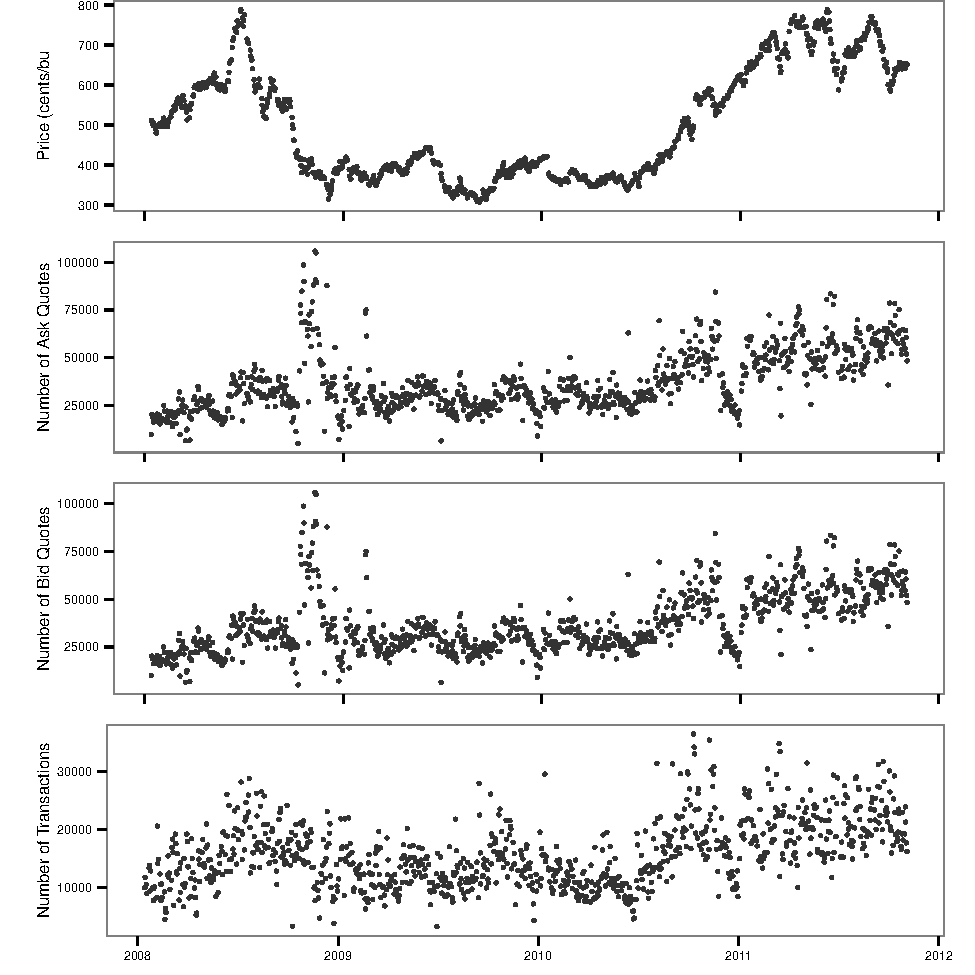
\includegraphics{TablesFigures_files/figure-latex/unnamed-chunk-3-1.pdf}
\caption{Price Levels, Number of Ask Quotes, Number of Bid Quotes, and
Number of Transactions}
\end{figure}

Figure displays data for the corn futures market from 1/14/2008 to
11/04/2011 for the nearby contract. The September contract is excluded
due to the possibility of `old crop' and `new crop' both being delivered
on this contract. To form the continuous nearby series contracts are
rolled to the next contract on the 20th of the month prior to the
delivery month.

\clearpage

\begin{figure}[htbp]
\centering
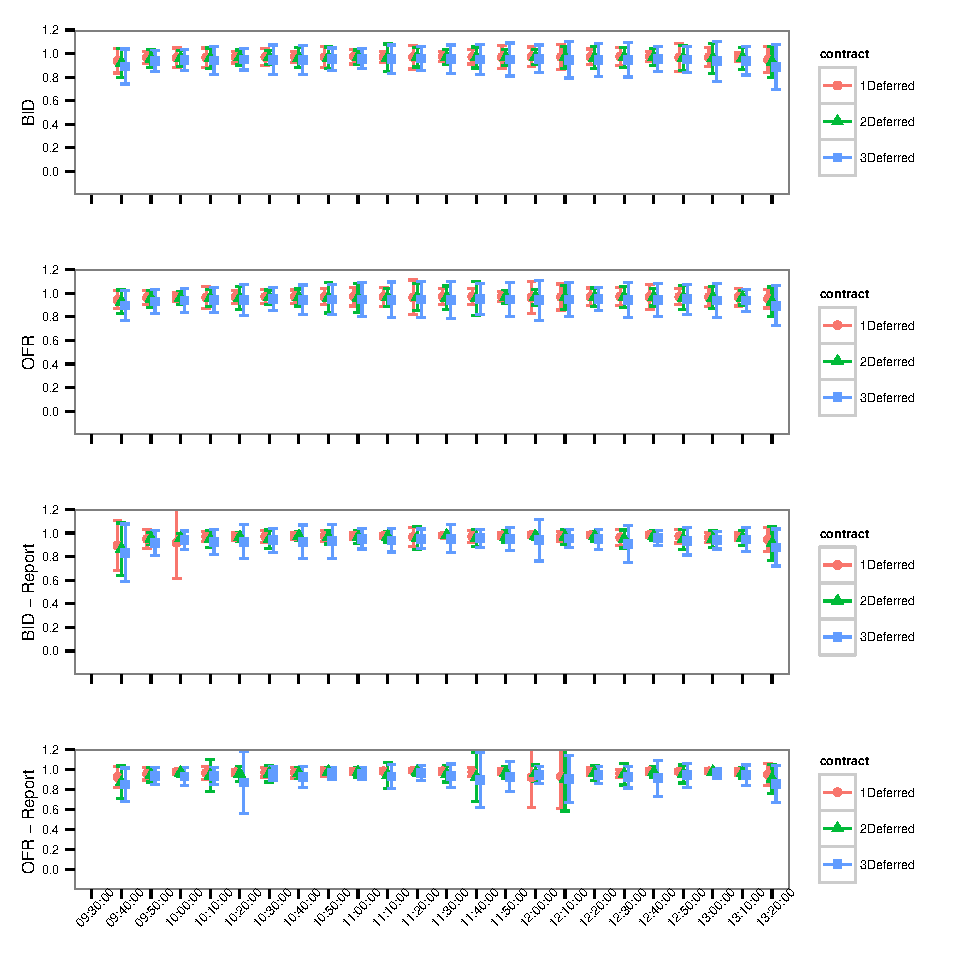
\includegraphics{TablesFigures_files/figure-latex/unnamed-chunk-4-1.pdf}
\caption{Information-Based Trading Activity and Contemporaneous
Correlations in the Top of the Book}
\end{figure}

Mean correlations and one standard deviation error bars over all days
are shown in the top two plots; report days only are included in the
bottom two plots.

\clearpage

\begin{figure}[htbp]
\centering
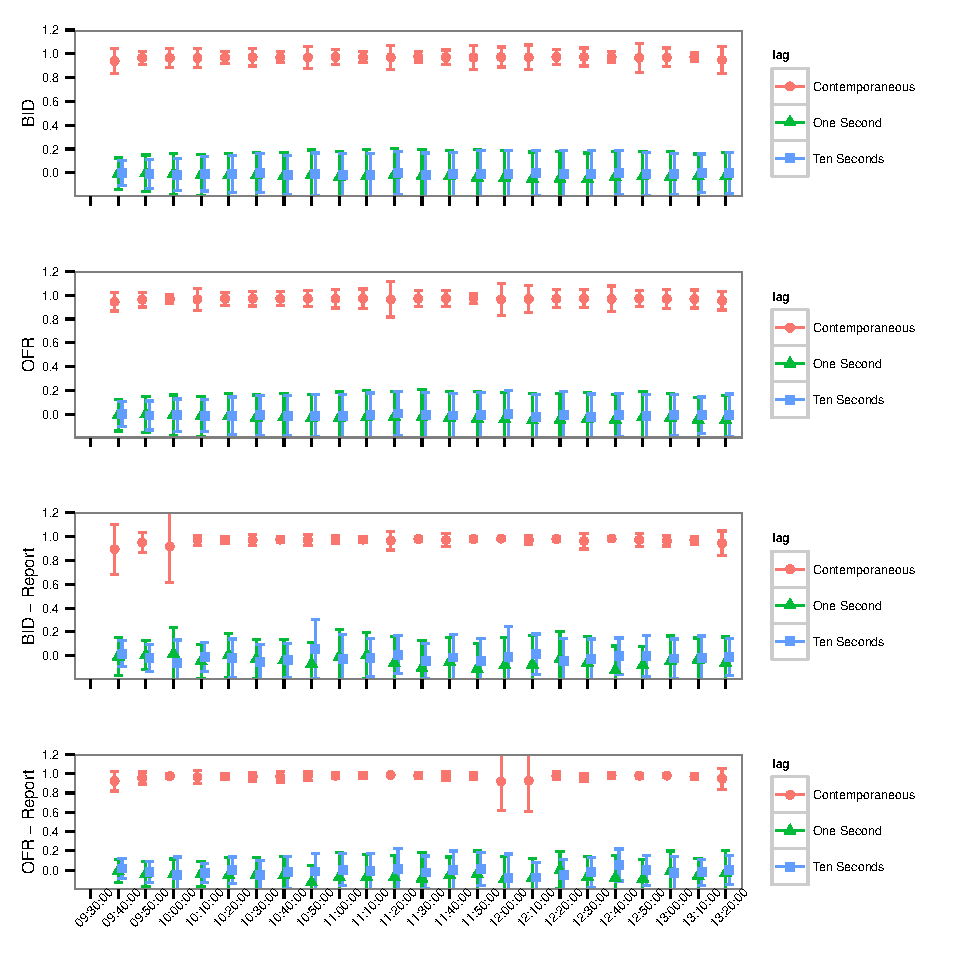
\includegraphics{TablesFigures_files/figure-latex/unnamed-chunk-5-1.pdf}
\caption{Speed of Information Transmission and Time-Lagged Correlations
in the Top of the Book}
\end{figure}

Mean correlations and one standard deviation error bars over all days
are shown in the top two plots; report days only are included in the
bottom two plots.

\clearpage

\begin{figure}[htbp]
\centering
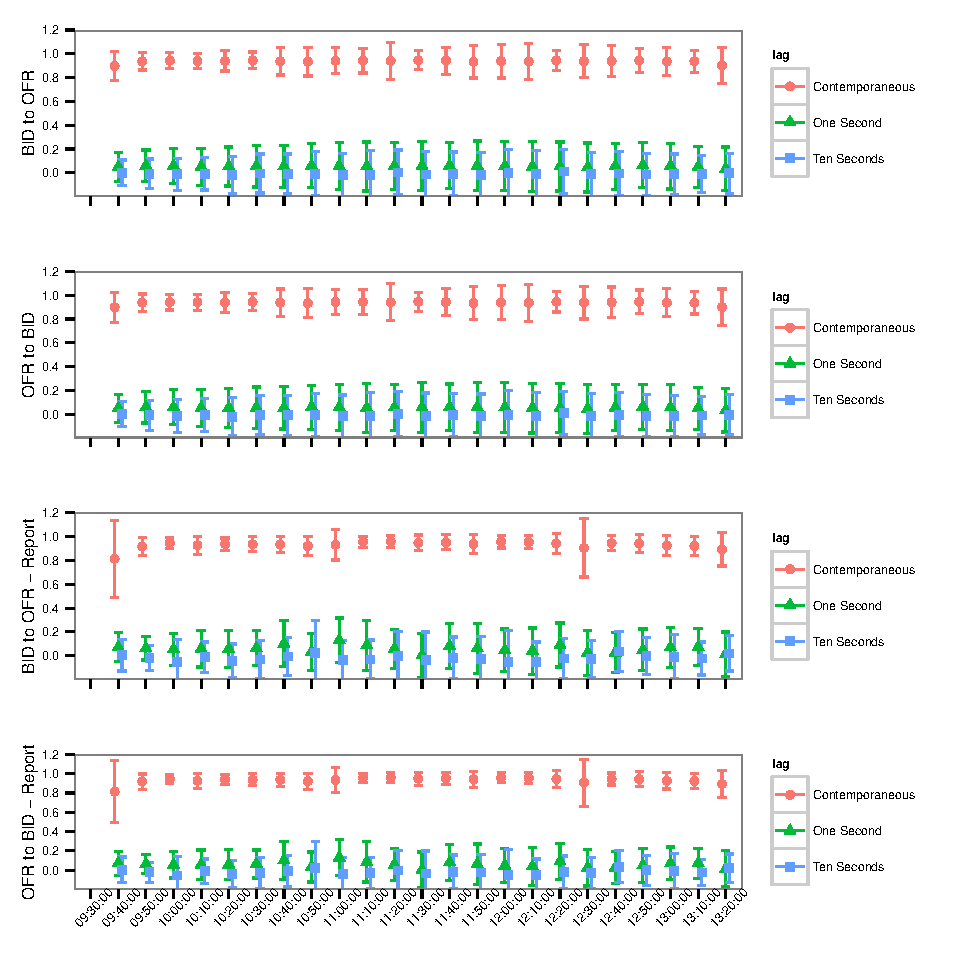
\includegraphics{TablesFigures_files/figure-latex/unnamed-chunk-6-1.pdf}
\caption{Spread Trades, Information Transmission, and Time-Lagged
Bid-to-Offer (Offer-to-Bid) Correlations}
\end{figure}

Mean correlations and one standard deviation error bars over all days
are shown in the top two plots; report days only are included in the
bottom two plots. Bid-to-Offer shows correlation between revisions to
the lagged nearby bid and the first deferred revisions to the offer, and
Offer-to-Bid shows correlation between revisions to the lagged nearby
offer and the first deferred revisions to the bid.

\end{document}
Status API Training Shop Blog About
© 2016 GitHub, Inc. Terms Privacy Security Contact Help